% !TEX root = ../Dokumentation.tex
\subsection{Energieversorgung}

\textbf{Funktionsbeschrieb}\\[0.2cm]
Das autonome Entsorgungsfahrzeug muss mit Energie versorgt werden. Dazu werden Akkumulatoren eingesetzt, welche das Gerät während dem gesamten Einsatz mit Strom versorgen. 
\\[0.2cm]
\textbf{Komponentenbeschrieb}\\[0.2cm]
\begin{figure}[h]
\centering
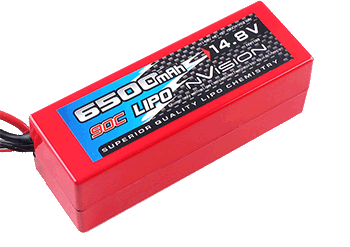
\includegraphics[width=0.5\textwidth]{03_Loesungskonzept/pictures/lipo.JPG}
\caption{2400 mA/h Lipo  (Quelle:http://www.conrad.ch/ce/)}	
\end{figure}\\[0.2cm]
Um Störungen, die z.B durch den erhöten Anlaufstrom der Motoren verursacht werden könnten, zu vermeiden, werden die intelligenten Systeme (Microcontroller, Mini-Computer,etc.)möglichst getrennt von den Motoren gespiesen. Dazu wird einerseits ein 11.1Volt Lithium-Polymer-Akkumulator für die Motoren verwendet und andererseits ein 7.4 Volt Lipo für die empfindlichen Systeme. Beide werden voraussichtliche eine Kapazität zwischen 1800 und 3000 mA/h vorweisen.
 \\[0.2cm]
\textbf{Begründung}\\
Lithium-Polymer-Akkumulatoren sind in einem vielfältigen Sortiment erhältlich und ermöglichen somit eine grosse Flexibilität was die Auswahl betrifft und beschleunigen damit auch die Suche nach einem Ersatz bei allfälligen Änderungen. Ausserdem zeichnen sich 
\textbf{Berechnungen}
\textbf{Testergebnisse}